\chapter{Návrh architektury}

Aplikace je rozdělena na serverovou a klientskou část. Server slouží pro odstínění klienta od RDF databází, komunikuje tedy přímo s datovými zdroji a zpracované data předává klientské aplikaci. Klient pak v případě potřeby z internetu stahuje externí obrázky (příkladem jsou konfigurace Wikidat, které obsahují URL odkazy) a autocomplete soubory.

Rozdělení aplikace na klient-server také umožňuje cachování na straně serveru, které ještě implementováno není. Tento problém je diskutován v poslední kapitole.

Server tak slouží na odstínění od link datové vrstvy a v budoucnu pro cachování dat, aktuálně je bezestavový.

\begin{figure}[h]
    \centering
    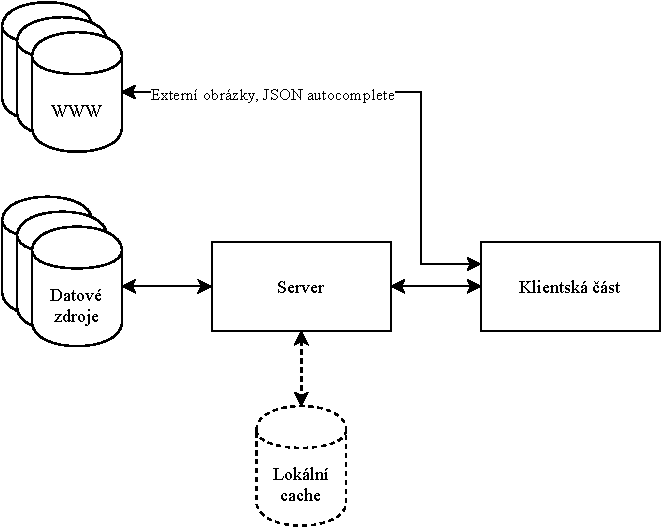
\includegraphics[width=0.75\textwidth]{media/communication.pdf}
    \caption{Komunikace mezi klientem, serverem a datovými zdroji. Cachování na serveru ještě implemontováno není.}
\end{figure}

\section{Server}
Jak již bylo v dokumentu zmíněno, převážná část serveru byla dodána jako specifikace pro klientskou aplikaci.

\subsection{Jazyková podpora} \label{jazykova-podpora}
Server jsem částečně přepsal, aby podporoval dotazování na data z více světových jazyků. Některé požadavky přijímají parametr \texttt{languages} obsahující čárkou (\texttt{,}) oddělené ISO 639-1 jazykové kódy. Server pak vrací objekty jejiž klíčem je jazykový kód a hodnotou daný překlad do jazyka. Pokud překlad neexistuje, hodnotou je \texttt{null}. V případě, že na všechny jazyky bylo vráceno \texttt{null}, server se pokusí přidat další jazyk, který existuje. Který jazyk takto bude vybrán není určeno.

Tato implementace umoňuje stahování vícejazyčných dat tak, že jsou stažené jen žádané jazyky, což může značně ušetřit přenos dat v některých případech, ale současně dojde ke stažení alespoň jednoho podporovaného jazyka, pokud je to možné.

\begin{prikl}
Pro \texttt{languages=cs,en} může server vrátit například
\begin{code}[frame=none]
{
    cs: null,
    en: "Kankakee County"
}
\end{code}
ale pokud nezná překlad ani do češtiny, ani do angličity, může vrátit
\begin{code}[frame=none]
{
    cs: null,
    en: null,
    sk: "Jazero Beňatina"
}
\end{code}
\end{prikl}

\subsection{API}
Server vrací data ve formátu JSON, požadavky jsou posílány metodou GET a parametry jsou kódovány do URL adresy.

\subsubsection{/metaconfiguration}
\textbf{parametry:} \texttt{iri} a \texttt{languages} \\
Vrátí informace o metakonfiguraci zadané podle \texttt{iri}. \\
Vrátí všechna data (viz kapitola \ref{pozadavky-metakonfigurace}) o metakonfiguraci, veškerá data o dceřiných konfiguracích (viz kapitola \ref{pozadavky-konfigurace}) a základní data o dceřiných metakonfiguracích (vše kromě seznamu konfigurací a metakonfigurací).

\begin{code}
interface ResponseMetaConfiguration extends
ResponseMetaConfigurationBase {
    has_meta_configurations: ResponseMetaConfigurationBase[],
    has_configurations: ResponseConfiguration[],
}

interface ResponseMetaConfigurationBase {
    iri: string,
    title: {[language: string]: string},
    description: {[language: string]: string},
    image: string,
}
\end{code}

\subsubsection{/configuration}
\textbf{parametry:} \texttt{iri} a \texttt{languages} \\
Vrátí informace o konfiguraci zadané podle \texttt{iri}. \\
Vrátí stejná data jako \texttt{/metaconfiguration} o svých sceřiných konfiguracích. \\
Toto volání se používá pouze když uživatel ručně zvolí IRI konfigurace, v opačném případě si aplikace vystačí s voláním \texttt{/metaconfiguration}.

\begin{code}
interface ResponseConfiguration {
    iri: string,
    stylesheet: string[],
    title: {[language: string]: string},
    description: {[language: string]: string},
    autocomplete: string[],
    starting_node: string[],
    resource_pattern: string|null,
}
\end{code}

\subsubsection{/stylesheet}
\textbf{parametry:} \texttt{stylesheet} \\
Vrátí kompletní visual style sheet (viz kapitola \ref{pozadavky-visual-style-sheet}) na základě jeho IRI jako parametr \texttt{stylesheet}.

\begin{code}
interface ResponseStylesheet {
    styles: {
        selector: string;
        properties: {
            [property: string]: string;
        }
    }[];
}
\end{code}

\subsubsection{/view-sets}
\textbf{parametry:} \texttt{config} a \texttt{resource} \\
Vrátí seznam možných view setů (viz kapitola \ref{pozadavky-view-sets}) které odpovídají uzlu s IRI \texttt{resource} při dané konfiguraci \texttt{config}.

\begin{code}
interface ResponseViewSets {
    viewSets: {
        iri: string;
        label: string;
        defaultView: string;
        views: string[];
    }[];
    views: {
        iri: string;
        label: string;
    }[];
}
\end{code}

\subsubsection{/preview}
\textbf{parametry:} \texttt{view} a \texttt{resource} \\
Vrátí data z dotazu preview (viz kapitola \ref{pozadavky-preview}) na uzel s IRI \texttt{resource} při daném pohledu \texttt{view}.

\begin{code}
interface ResponsePreview {
    nodes: ResponseElementNode[];
    types: ResponseElementType[];
}
\end{code}

\subsubsection{/detail}
\textbf{parametry:} \texttt{view} a \texttt{resource} \\
Vrátí data z dotazu detail (viz kapitola \ref{pozadavky-detail}) na uzel s IRI \texttt{resource} při daném pohledu \texttt{view}.

\begin{code}
interface ResponseDetail {
    nodes: {
        iri: string;
        data: {
            [IRI: string]: string;
        };
    }[];
    types: ResponseElementType[];
}
\end{code}

\subsubsection{/expand}
\textbf{parametry:} \texttt{view} a \texttt{resource} \\
Vrátí expandované uzly (viz kapitola \ref{pozadavky-expansion}) pro uzel s IRI \texttt{resource} při daném pohledu \texttt{view}. Tyto expandované uzly již obsahují data o detailu a tedy není třeba žádného dalšího volání.

\begin{code}
interface ResponseExpand {
    nodes: ResponseElementNode[];
    edges: ResponseElementEdge[];
    types: ResponseElementType[];
}
\end{code}

\newpage

Mezi pomocná rozhraní pak patří
\begin{code}
interface ResponseElementType {
    iri: string;
    label: string;
    description: string;
}

interface ResponseElementEdge {
    source: string;
    target: string;
    type: string;
    classes: string[];
}

interface ResponseElementNode {
    iri: string;
    type: string;
    label: string;
    classes: string[];
}
\end{code}

\begin{figure}[p]
    \centering
    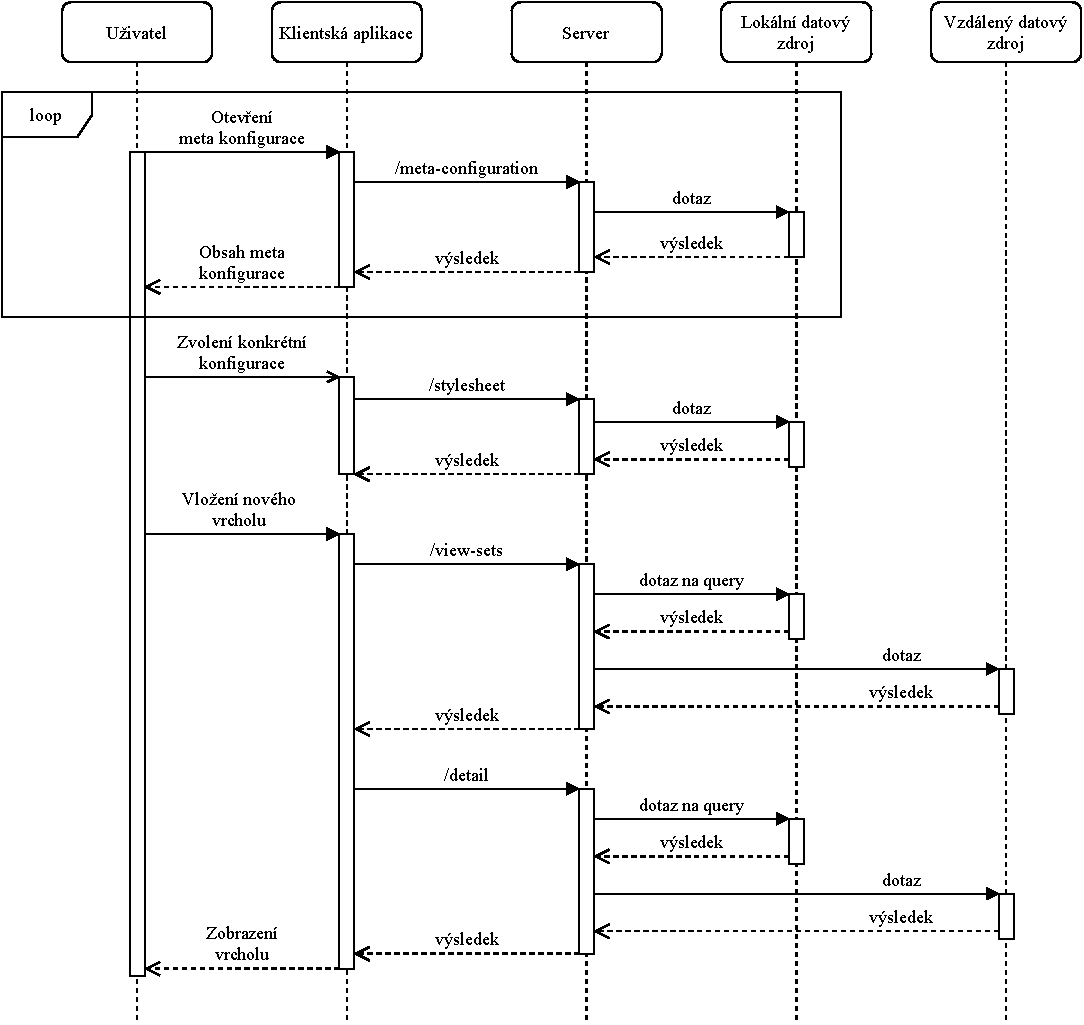
\includegraphics[width=\textwidth]{media/sequence-server.pdf}
    \caption{Schéma komunikace se serverem a RDF databází při spuštění aplikace. Nejprve klient vybírá konfiguraci. Poté začne stahování stylesheetu a stahování prvního vrcholu. Nejprve se stáhnout \texttt{view-sets} a poté z výchozího pohledu se stáhne \texttt{detail} a vrchol se zobrazí na grafu.}
\end{figure}


\section{Klient}

\begin{figure}
    \centering
    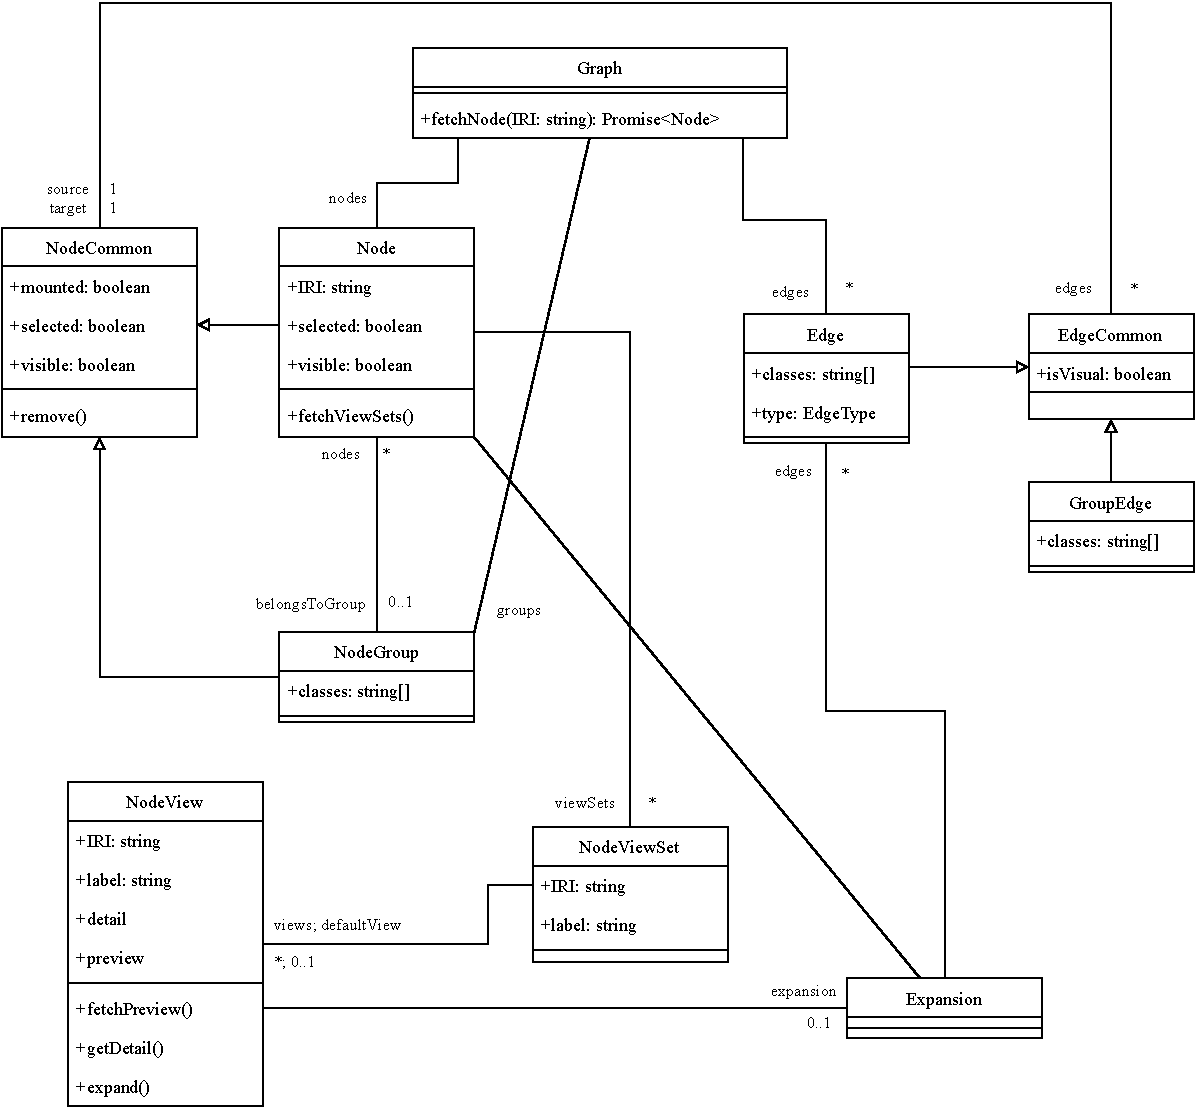
\includegraphics[width=\textwidth]{media/graph.pdf}
    \caption{Class diagram části aplikace jež pracuje s grafem.}
\end{figure}

\subsection{Moduly}

\subsubsection{Připojení na server}
Tento modul řeší komunikaci se serverem.

\subsubsection{Graf}
Tato část aplikace reprezentuje stažený graf a všechny jeho data. Má metody pro práci s grafem, jeho modifikaci a stahování nových dat ze serveru.

\subsubsection{Filtrování}
Tento modul integruje možnost filtrování vrcholů v aplikaci na základě různých grafových a sémantických vlastností. Modul se dá rozšířit o další filtry i za runtime a nabízí tedy možnost instalace pluginů.

\subsubsection{Layoutování}
Modul řeší uspořádání vrcholů v grafu. Layoutování reaguje na významné události z grafu. Jedná se například o vložení nového vrcholu, expanzi, přesunutí vrcholů, zamčení vrcholů atp. Stejně jako filtrování, jednotlivé layouty lze přidávat za runtime a je tedy možné s pomocí pluginů přidat nové layouty.

\subsubsection{Vyhledávání}
Modul vyhledávání vrací vrcholy na základě textového řetězce. Vyhledává v grafu, z autocomplete nebo se pokusí IRI sestavit z hledaného výrazu. Jednotlivé vyhledávače lze rozšířit o další stejně jako u filtrování a layoutování.

\subsubsection{Ukládání do souboru}
Řeší jak uložit a znova načíst stav aplikace do a ze souboru.